\newpage

\chapter{Electronics Design}

Electronics section overview ...

\newpage

\section{Sensors}

Speed sensors are required to measure the rotational speed of the two rear drums. For the application, RPR-220 infrared photoreflectors were used as they allow for reliable contactless speed measurements. The RPR-220 unit was also readily available, inexpensive and would work with the Raspberry Pi's \acs{gpio} pins.

Sensors are required to measure the angular velocity of both the rear cylinders. It was decided that using a infrared transmitter-receiver device with reflective strips on the cylinder would be sufficient. The sampling rate of the sensors should be high enough to gather high resolution measurements, but should remain accurate up to the maximum expected drum speed.

The raspberry Pi is capable of measuring inputs using the standard Rpi.GPIO library up to \SI{5}{\kilo\hertz}. Since the maximum expected drum rotation speed is 3500 \acs{rpm}, which equates to \SI{66.6}{\hertz}, the sensors would be capable of handling up to 75 segments per revolution. Considering a safety factor and in order to reduce the data burden, a sensor system implementing 60 segments was selected to ensure high enough resolution at low speeds.

\begin{table}[h!]
	\renewcommand{\arraystretch}{1.5}
	\centering
	\caption{RPR-220 Data Sheet Parameter Summary}
	\citep{RPR:2015}
	\begin{tabularx}{\textwidth}{X >{\raggedright}p{3cm} >{\raggedright\arraybackslash}p{2cm} }
		\toprule
		Parameter                       & Condition & Value                   \\
		\midrule
		LED Current                     & Maximum   & \SI{50}{\milli\ampere}  \\
		LED Voltage                     & Rated     & \SI{5}{\volt}           \\
		Phototransistor Current (Dark)  & Rated     & \SI{0.5}{\micro\ampere} \\
		Phototransistor Current (Light) & Rated     & \SI{0.8}{\milli\ampere} \\
		Phototransistor Response Time   & Rated     & \SI{10}{\micro\second}  \\
		\bottomrule
	\end{tabularx}
	\label{tab:rprdata}
\end{table}

\begin{figure}[h!]
	\centering
	\begin{subfigure}[t]{.315\textwidth}
		\centering
		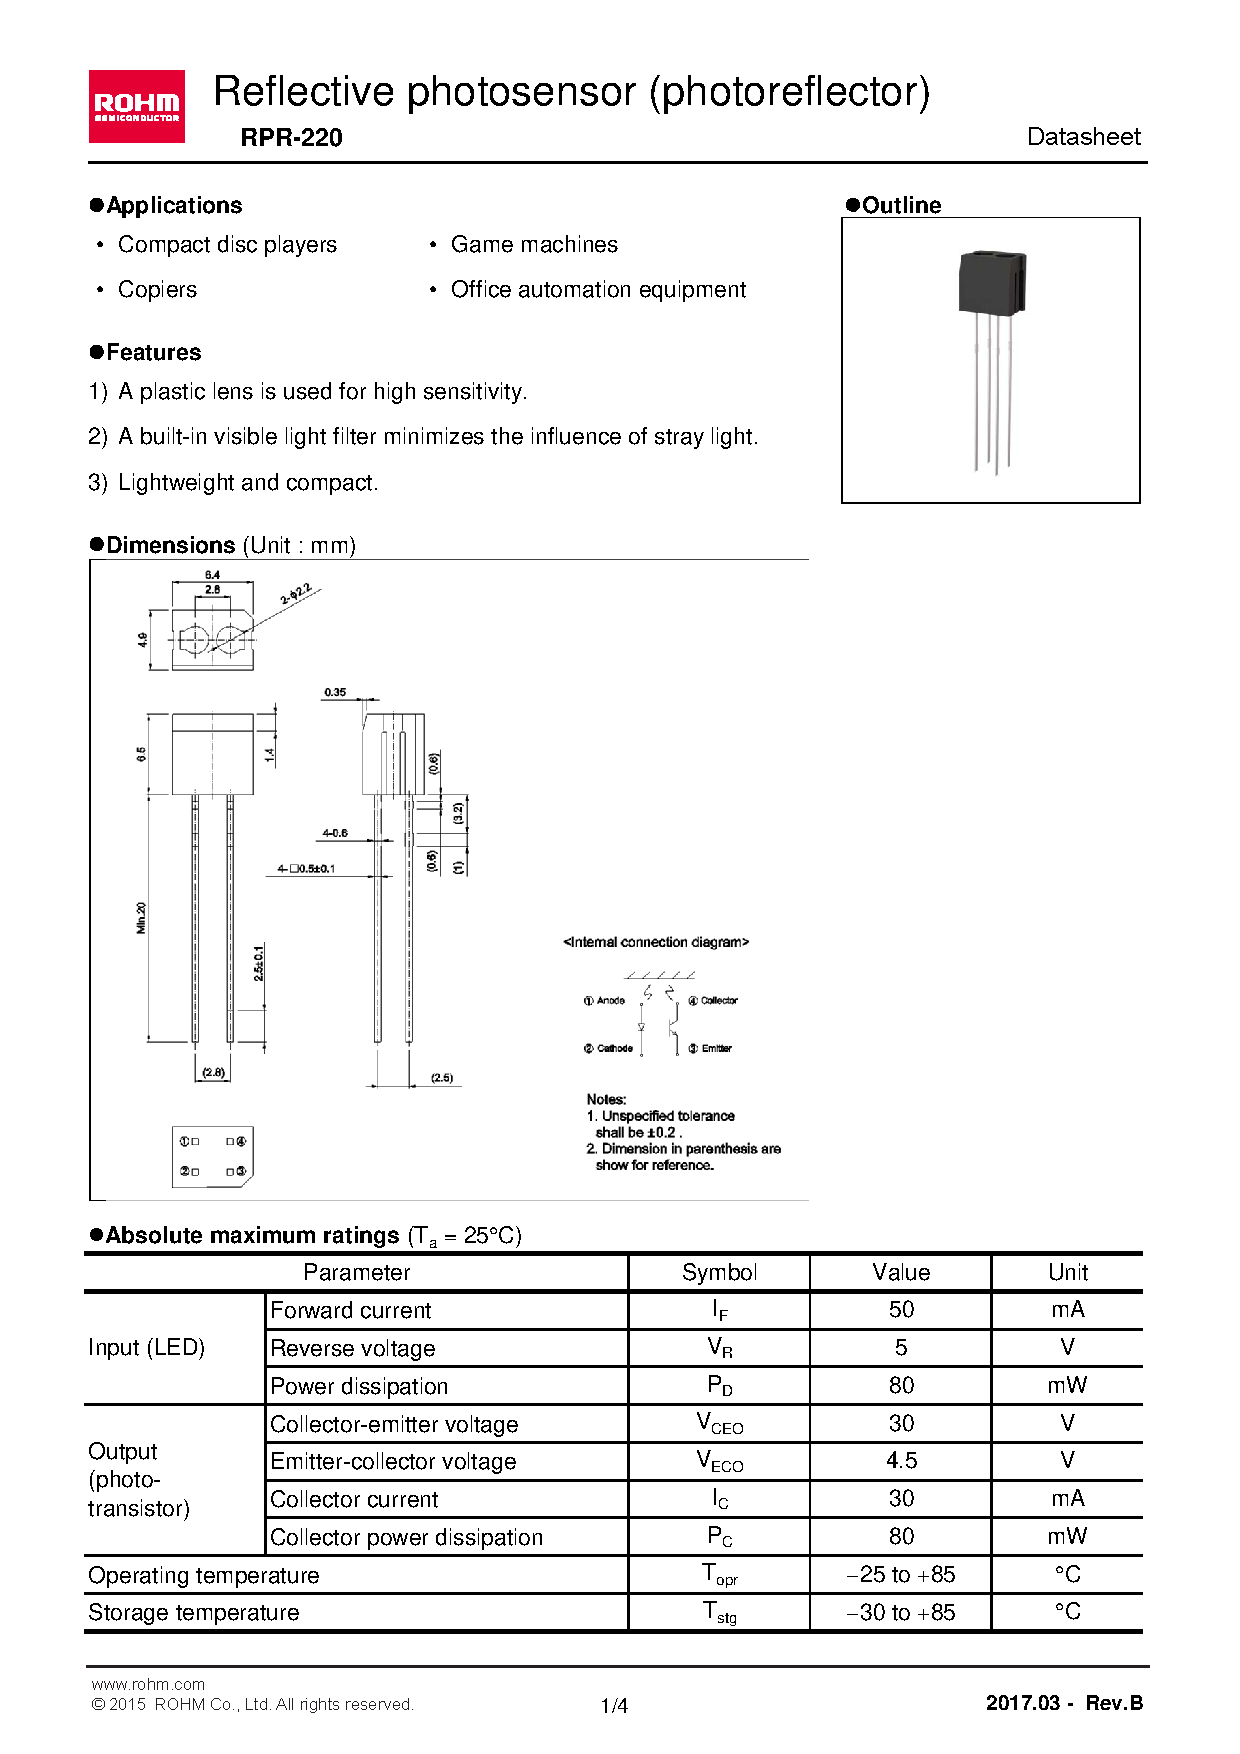
\includegraphics[width = \linewidth]{RPR220.jpg}
		\caption{RPR-220 Photoreflector}
		\citep{RPR:2015}
		\label{fig:rpr}
	\end{subfigure}
	\begin{subfigure}[t]{.65\textwidth}
		\centering
		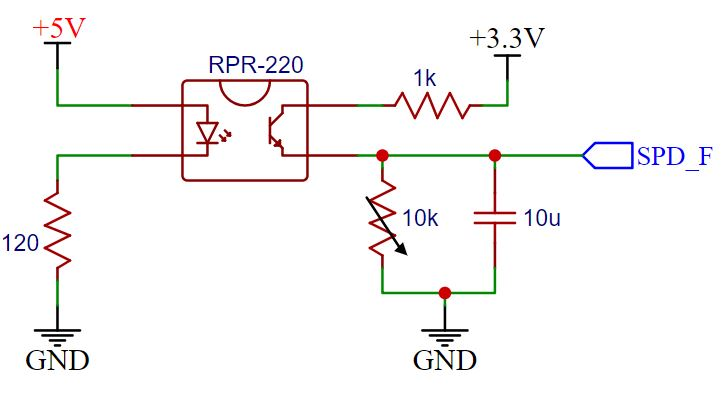
\includegraphics[width = \linewidth]{SensorCircuit.JPG}
		\caption{Sensor Biasing and Filter Circuit}
		\label{fig:sensorD}
	\end{subfigure}
	\caption{Sensor Implementation}
	\label{fig:Sensor}
\end{figure}


\begin{equation}
	f_c = \frac{1}{2 R C}
\end{equation}

\newpage


\section{Motor Control}

\begin{figure}[h!]
	\centering
	\begin{subfigure}[t]{.550\textwidth}
		\centering
		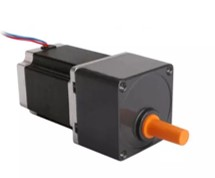
\includegraphics[height = 3cm]{StepperMotor.jpg}
		\caption{Nema 23 Stepper Motor with 15:1 Gearbox}
		\citep{Robotics:2022}
		\label{fig:stepper}
	\end{subfigure}
	\begin{subfigure}[t]{.41\textwidth}
		\centering
		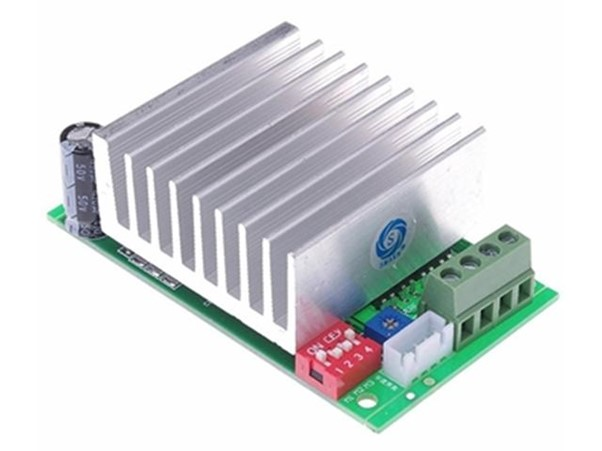
\includegraphics[height = 2.5cm]{StepperDriver.jpg}
		\caption{TB660 v1.1 Stepper Motor Driver}
		\citep{Communica:2022}
		\label{fig:motorDriver}
	\end{subfigure}
	\caption{Motor Control Components}
	\label{fig:Motor}
\end{figure}



After testing the resistance level between the wires on the Nema-23 stepper motor, the results were:

\begin{table}[h!]
	\centering
	\caption{Stepper Motor Wire Resistance Measurement Results}
	\begin{tabularx}{\textwidth}{X X X X X X  }
		\toprule
		       & Black               & Green               & Red                 & Yellow              & White           \\
		\midrule
		Blue   & > \SI{1}{\mega\ohm} & > \SI{1}{\mega\ohm} & \SI{41.2}{\ohm}     & > \SI{1}{\mega\ohm} & \SI{20.7}{\ohm} \\
		White  & > \SI{1}{\mega\ohm} & > \SI{1}{\mega\ohm} & \SI{20.8}{\ohm}     & > \SI{1}{\mega\ohm} &                 \\
		Yellow & \SI{20.7}{\ohm}     & \SI{20.5}{\ohm}     & > \SI{1}{\mega\ohm} &                     &                 \\
		Red    & > \SI{1}{\mega\ohm} & > \SI{1}{\mega\ohm} &                     &                     &                 \\
		Green  & \SI{40.5}{\ohm}     &                     &                     &                     &                 \\
		\bottomrule
	\end{tabularx}
	\label{tab:nemaTest}
\end{table}

From Table \ref{tab:nemaTest} above, the wires associated with each coil can be identified. A resistance of > \SI{1}{\mega\ohm} indicates that the wires are not connected to the same coil. For the wires on the same coil, a larger resistance indicates that there is more coiled wire between the connections, and they are thus farther apart. This results in the :

\begin{figure}[h!]
	\begin{center}
		
\includegraphics[width=0.3\textwidth]{MotorWire.jpg}
		\caption{Nema-23 Wiring}
		\label{fig:motorWire}
	\end{center}
\end{figure}
